\section{Análisis del Problema}

El problema a resolver consiste en crear un servidor de música y un cliente 
que logren comunicarse entre sí, de manera que el cliente pueda reproducir
la música que el servidor ofrece, en forma de streams de audio. El servidor 
por su parte debe ser capaz de administrar la lista de canciones disponibles
para reproducir, así como almacenar las canciones para su posterior
reproducción. Por último, el servidor debe ser capaz de atender a múltiples
clientes de manera concurrente. Todo esto utilizando el lenguaje de programación
Go.

Por otro lado, el cliente debe ser capaz de realizar consultas al servidor para
obtener la lista de canciones disponibles, así como también debe permitir la
creación de listas de reproducción locales. El cliente debe tener la capacidad
de reproducir la música que el servidor ofrece. Asimismo, el cliente debe 
ofrecer una interfaz gráfica que permita al usuario interactuar con el
programa de manera intuitiva. Estas funcionalidades deben ser implementadas
utilizando el lenguaje de programación F\#.

Los requerimientos funcionales del servidor son los siguientes:

\begin{itemize}
    \item Atender a múltiples clientes de manera concurrente.
    \item Administrar la lista de canciones disponibles para reproducir.
    \item Almacenar las canciones para su posterior reproducción.
    \item El servidor debe ser capaz servir las canciones a los clientes.
\end{itemize}

Los requerimientos funcionales del cliente son los siguientes:

\begin{itemize}
    \item Ofrecer una interfaz gráfica para la interacción con el usuario.
    \item Realizar consultas al servidor para obtener la lista de canciones.
    \item Crear listas de reproducción locales.
    \item Reproducir la música que el servidor ofrece, manteniendo un buffer 
    de reproducción.
    \item Permitir filtrar las canciones por al menos 3 criterios distintos.
\end{itemize}

De esta manera, se puede concluir cuales son los criterios y requerimientos
a cumplir para la realización del proyecto. En la siguiente sección se
presenta la solución propuesta para el problema.

\section{Solución del Problema}

Durante el desarrollo del proyecto se implementaron dos programas, un servidor
y un cliente. Cada uno cuenta con características y funcionalidades distintas,
las cuales se proceden a describir a continuación.

\subsection{Servidor}

Tomando como base los requerimientos establecidos para el servidor, se
implementó un programa que cumple con las siguientes características:

\subsubsection{Concurrencia}

El servidor es capaz de atender a múltiples clientes por medio de la
implementación de procesos en paralelo. Para lograr esto, se hace uso de las 
goroutines de Go, las cuales permiten la ejecución de funciones de manera
concurrente. De esta manera, cada vez que un cliente se conecta al servidor,
se crea una goroutine que se encarga de atender al cliente. Lograndose así
la concurrencia por parte del servidor.

\subsubsection{Administración de la lista de canciones}

Para la administración de la lista de canciones, se implementó una base de 
datos del lado del servidor, utilizando SQLite. De esta manera, el servidor
es capaz de almacenar las canciones que recibe de los clientes, así como
también es capaz de administrar la lista de canciones disponibles para
reproducir. Almacenando información como el nombre de la canción, el artista,
la duración, el género, un hash (del cual se hablará más adelante) y una flag 
que indica si la canción está disponible para reproducir.

\subsubsection{Almacenamiento de las canciones}

El almacenamiento de las canciones está muy ligado a como se transmite la
música entre el servidor y el cliente. Las canciones se reciben como un archivo 
de audio en formato MP3, el cual es transformado a un formato utilizado por el 
protocolo HLS, el cual es un protocolo de streaming de audio y video. Este
protocolo divide el archivo de audio en pequeños segmentos, los cuales son
almacenados en el servidor. Estos archivos se almacenan bajo un directorio
con el Hash de la canción, el cual es calculado utilizando el nombre y artista 
de la canción. De esta manera, se puede identificar de manera única cada
canción almacenada en el servidor.

\subsubsection{Servir las canciones}

Como se mencionó anteriormente, las canciones se almacenan en el servidor
utilizando el protocolo HLS. Según \cite{cloudflare} HTTP Live Streaming (HLS) es:

\begin{quote}
    "uno de los protocolos de transmisión de video más utilizados. Aunque se
    denomina transmisión "en vivo" HTTP, se utiliza tanto para transmisión bajo
    demanda como para transmisión en vivo. HLS divide los archivos de vídeo en
    archivos HTTP descargables más pequeños y los entrega mediante el protocolo
    HTTP. Los dispositivos cliente cargan estos archivos HTTP y luego los
    reproducen como video."
\end{quote}

Si bien este protocolo está diseñado para la transmisión de video, también
puede ser utilizado para la transmisión de audio. HLS ofrece un sistema de 
transmisión robusto y con un buffer de almacenamiento. De esta manera, el
servidor es capaz de servir las canciones a los clientes utilizando el protocolo
HLS.

Se tomó la decisión de obviar la indicación de utilizar TCP como protocolo 
principal para la comunicación entre el servidor y el cliente, ya que el
protocolo HLS ofrece un sistema de transmisión más realista y funcional
con respecto al desarrollo de un sistema de streaming de música.

\subsection{Cliente}

Tomando como base los requerimientos establecidos para el cliente, se
implementó un programa que cumple con las siguientes características:

\subsubsection{Interfaz gráfica}

El cliente cuenta con una interfaz gráfica desarrollada utilizando el framework
Avalonia tal como se muestra en la figura \ref{fig:app}. Este framework permite
el desarrollo de interfaces gráficas multiplataforma utilizando el lenguaje de
programación F\#. La interfaz gráfica del cliente cuenta con las siguientes
características:

Una barra de búsqueda que se puede usar para buscar canciones, un menú
desplegable que se puede usar para filtrar las canciones por género y un filtro
de duración que se puede usar para filtrar las canciones por duración. Es
importante señalar que cada filtro es independiente, por lo que si filtras por
género y luego por duración, solo se aplicará el filtro de duración.

El cliente tiene una pestaña Canciones y Lista de reproducción a la izquierda,
la pestaña Canciones muestra todas las canciones que coinciden con los filtros o
Listas de reproducción, y la pestaña Lista de reproducción muestra todas las
listas de reproducción que se han creado. Cuando se slecciona una lista de
reproducción, el usuario se debe cambiar a la pestaña Canciones para ver las
canciones de la lista de reproducción.

A la derecha, hay una barra de herramientas que se puede usar para actualizar
los filtros de canciones en la pestaña de canciones y, en la pestaña de lista de
reproducción, se puede usar para crear una nueva lista de reproducción.

Cada elemento de la pestaña Canciones y lista de reproducción tiene un menú
contextual que se puede utilizar para acciones específicas. Se puede acceder
haciendo clic derecho en el elemento. En la pestaña de canciones, el menú
contextual tiene las opciones para agregar o eliminar la canción de una lista de
reproducción, y en la pestaña de la lista de reproducción, el menú contextual
tiene las opciones para eliminar una lista de reproducción.

En la parte inferior hay un reproductor que sirve para reproducir las canciones.
El reproductor tiene los controles básicos, reproducir, pausar, siguiente y
anterior. También tiene un control deslizante para el volumen y un control
deslizante para el progreso de la canción. En la parte superior de estos
controles, hay una etiqueta que muestra la canción actual y el artista de la
canción.

\begin{figure}
    \centering
    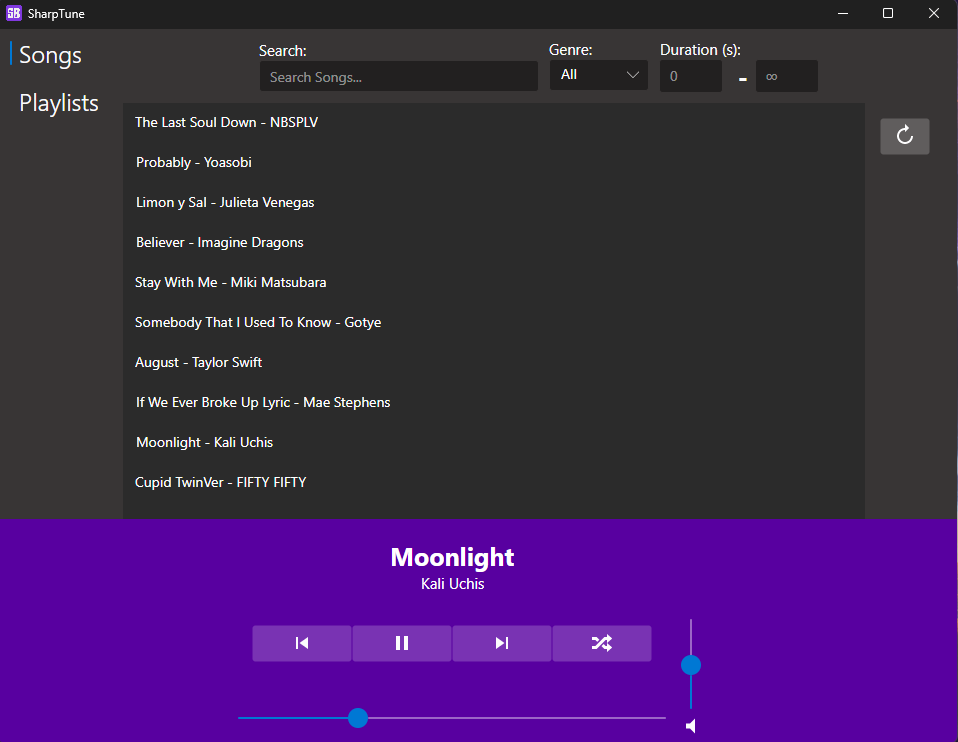
\includegraphics[width=3in]{assets/app.png}
    \caption{Interfaz gráfica del cliente}
    \label{fig:app}
\end{figure}

\subsubsection{Consultas al servidor}

Debido a que el servidor utiliza HLS, el cual está basado en el protocolo HTTP,
el cliente realiza consultas al servidor utilizando el protocolo HTTP. De esta
manera, el cliente es capaz de obtener la lista de canciones disponibles para
reproducir, así como también es capaz de obtener las canciones que el usuario
solicite.

\subsubsection{Creación de listas de reproducción locales}

El cliente es capaz de crear listas de reproducción locales, las cuales son
almacenadas en una base de datos SQLite. De esta manera, el cliente es capaz de
almacenar las listas de reproducción que el usuario cree, así como también es
capaz de almacenar las canciones que el usuario agregue a las listas de
reproducción.

\subsubsection{Reproducción de música}

Para la reproducción de música, el cliente utiliza el protocolo HLS. Por lo cual 
se utiliza LibVLC para reproducir las canciones en Windows y LibVLCSharp para
reproducir las canciones en Linux. De esta manera, el cliente es capaz de
reproducir las canciones que el servidor ofrece. Por medio de estas librerías,
el cliente es capaz de mantener un buffer de reproducción, el cual permite
reproducir las canciones sin interrupciones y teniendo la posibilidad 
de pausar, adelantar o retroceder la reproducción de la canción.

\subsubsection{Filtrado de canciones}

El cliente es capaz de filtrar las canciones por nombre|artista, género y
duración. De esta manera, el cliente es capaz de mostrar al usuario las
canciones que coincidan con los filtros aplicados. Tal como se mencionó
anteriormente, los filtros son independientes, por lo que si se filtra por
género y luego por duración, solo se aplicará el filtro de duración.